%Préambule
\documentclass[12pt]{report}

\usepackage[french]{babel}
\usepackage{luatextra}
\usepackage{hyperref}
\usepackage{hhline}
\usepackage{multirow}
\usepackage{listings}
\usepackage{caption}
\usepackage{amsmath}

\usepackage{lastpage}

\usepackage{fancyhdr}


\pagestyle{fancy}

\renewcommand{\thesection}{\Roman{section}}

%Information sur le document
\title{Projet: Ascenseur}
\date{16 juin 2019}
\author{Victor \textsc{ALAIN} \& Arthur \textsc{BLAISE} \& Amélie \textsc{GUEDES} \\ \& Loann \textsc{POTTIER}}

 \makeatletter
\let\theauthor\@author
\let\thetitle\@title
\let\thedate\@date
\makeatother

%En-tête
\fancyhead[C]{}
\fancyhead[L]{\leftmark}
\fancyhead[R]{\rightmark}

%Pied-de-Page
\fancyfoot[C]{\thepage\ / \pageref{LastPage}}
\fancyfoot[R]{\thetitle}
\fancyfoot[L]{\thedate}

\begin{document}

\maketitle
\tableofcontents

\clearpage


\section{Introduction}

\subsection{Démarrage et explication}
	Tout d'abord nous avons décidé de jouer concrètement au jeu, afin d'essayer de comprendre les règles pour mis cerner les problèmes que l'on peut rencontrer en créant les algorithmes. Notre principal problème de compréhension dans le jeu était comment fonctionnent les atouts quels sont-ils et quelles cartes jouer et à quel moment. Ainsi, nous avons fait une partie et nous sommes parvenus à comprendre les principales règles de l'Ascenseur sans comprendre totalement comment fonctionnait le décompte des points. Cela nous a également permis de nous imaginer une schématisation de ce qu'on nous demandait de faire dans une grande globalité. Puis on a pris conscience des consignes qui était les suivantes:
	
\subsection{Problèmes à résoudre}
	
	Le but de ce projet est de réaliser un algorithme permettant d'exécuter le jeu l'Ascenseur. Pur ce faire, plusieurs consignes nous ont été donné(?): 
	\begin{itemize}
		\item  {Tout d'abord, nous devont réaliser un algorithme nommé "100\% humain" où il faut 
		initialiser certains paramètre notamment le nombre de joueurs (et donc le nombre de cartes maximal et par manche) puis l'utilisation des atouts et enfin les modalités de victoires et de défaites, en fixant le nombre de points gagnés par défaut, par plis remportés et les points perdus dans les deux mêmes catégories. Ensuite, il faut réaliser l'algorithme qui permet de jouer au jeu de l'ascenseur avec les deux phases : ascendente et descendante. Pour ce faire, il faut indiquer le nombre de manche par phase (Qui varie en fonction du nombre de joueur) et du nombre de tours par manches. Il faut également prendre en considération le fait que chaque cartes jouées est remis en bas du packet de cartes initiales c'est à dire qu'une carte sera jouées plusieurs fois dans la même partie. De plus, il faut que la distribution suivent un nombre logique (Dans le sens des aiguilles d'une montre notamment). En distribuant on finit toujours de distribuer par le joueur situé juste avant le joueur qui a reçu la 1ère carte. On doit également compter le nombre de points réaliser par chaque jour et donc, il faut, après chaque distribution avant de commencer la manche, que le joueur dise à haute voix le parie qu'il soit réalisé. \\ De surcroît, chaque jour ayant remporté le tour précédement, commence au tour suivant. Il est important également que chaque joueur jouent une carte de la couleur demandée si il en possède une, sinon il doit jouer un atout. Cependant, un joueur n'est pas obligé un atout si il n'a pas de carte de la même couleur, il peut déposer une carte quelconque mais il perdra le tour.
A la fin de la partie, le joueur possédant le plus de point à l'aide des contracts/paris gagnent la partie.  Attention, les jokers ne font pas partie du jeu.}
		\item {Dans un second temps, on va créer un algorithme nommé "Version'Ordinateur'" qui reprendra l'algorithme précédent mais qui va implémenter des joueurs artificiels, qui devront chercher à gagner à tout prix (Il s'agit donc d'une IA qui aura les mêmes pensées qu'un humain). On devra considérer une IA comme un humain, c'est-à-dire qu'il jouera exactement la même chose que ce que l'homme jouerai. } \\
		\\
	
	\begin{figure}
	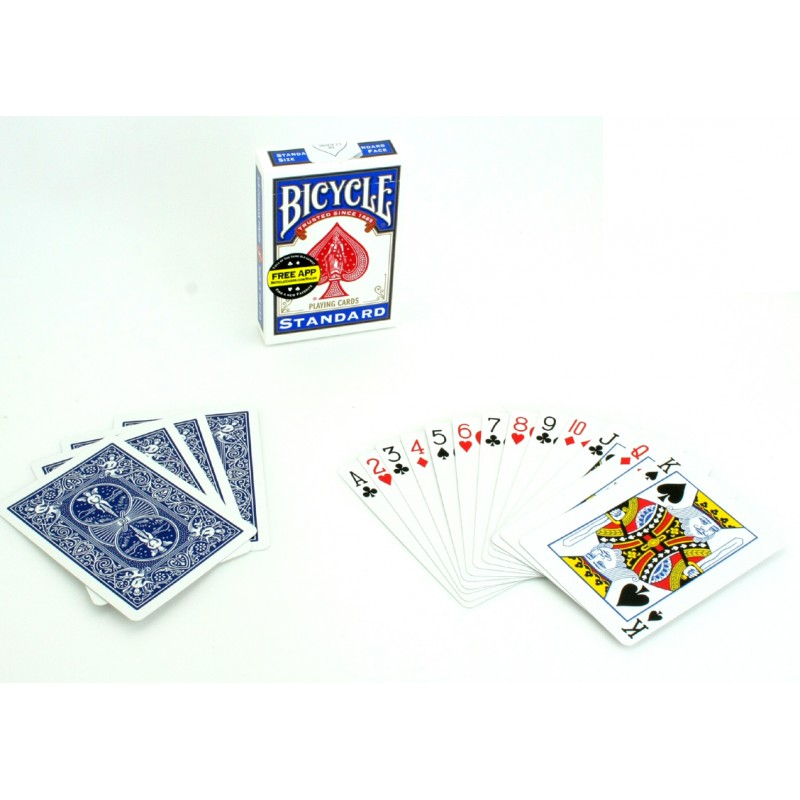
\includegraphics[scale=0.30]{jeu-de-cartes-magicien-bicycle-stripper.jpg}
	 \caption{Jeu de carte utilisé lors d'une partie d'ascenseur}
	\end{figure}
		

		
\clearpage

		
\section{Explication des algorithmes}

\section{Diffultés et conclusion}
			
	\end{itemize}
\end{document}
